%\documentclass[../main/6103-LecturesNotes.tex]{subfiles}
%\begin{document}

\section{Trigonometric functions} 
\subsection{Measuring angles}
\begin{definition}[Degrees]
Degrees are defined so that one full turn is $360$\degs.
\end{definition}

\begin{definition}[Radians]
Radians (usually abbreviated as rad or \rads) are defined using a circle of radius $1$. The angle between two radii in the unit circle in radians is equal to the arc length between the two radii.
\end{definition}

\begin{figure}[H]
    \centering
    \subfigure[{$360^{\circ}$ is a full turn.}]{\label{fig:360-turn}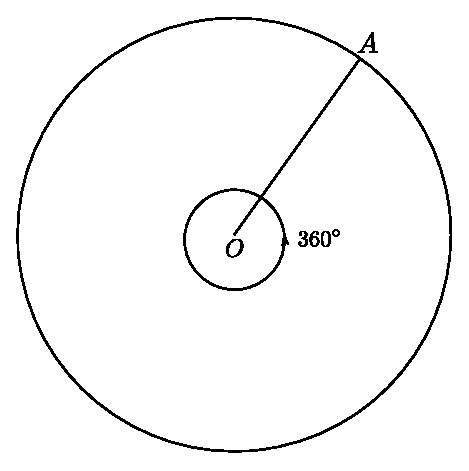
\includegraphics[scale=0.6]{img/360-turn}}
    \hspace{2.0cm}
    \subfigure[{A unit circle with angles of $s$\rads\ and $t$\rads\ marked.}]{\label{fig:s+t-angels}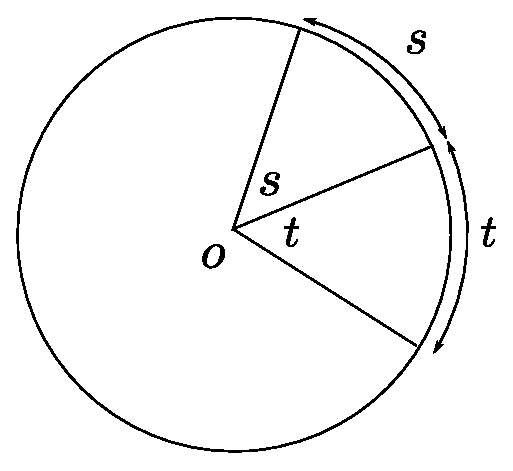
\includegraphics[scale=0.6]{img/s+t-angels}}
    \label{fig:exponent-graphs}
\end{figure}

We can see immediately that a full turn is $2\pi\,\mbox{rad}$ because a circle of radius $1$ has a circumference $2\pi$. Therefore we have
\begin{in_a_box}
$$\begin{array}{rcccl}
1\text{ turn}&=&360^{\circ}&=&2\pi\,\mbox{rad}\\
\frac{1}{2}\text{ turn}&=&180^{\circ}&=&\pi\,\mbox{rad}
\end{array}$$
\end{in_a_box}
So,
\begin{in_a_box}
\begin{eqnarray*}
1\,\mbox{rad}&=&\frac{180}{\pi}^{\circ}\\
1^{\circ}&=&\frac{\pi}{180}\,\mbox{rad}\\
\end{eqnarray*}
\end{in_a_box}
If the radius is not $1$, then you need to take the ratio 
\begin{equation}
\frac{\text{arc length}}{\text{radius}} = \text{angle (in radians)}.
\end{equation}

\subsection{Trignometric functions: cosine, sine \& tangent}\label{trig-functions}
\begin{definition}[sin, cos and tan]
The values $\cos(\theta)$ and $\sin(\theta)$ (often written $\cos\theta,\, \sin\theta$) are the horizontal and vertical coordinates of the point $C$. $\tan(\theta)$ (often $\tan\theta$) is defined to be $\frac{\sin\theta}{\cos\theta}$.

\begin{figure}[H]
\centering
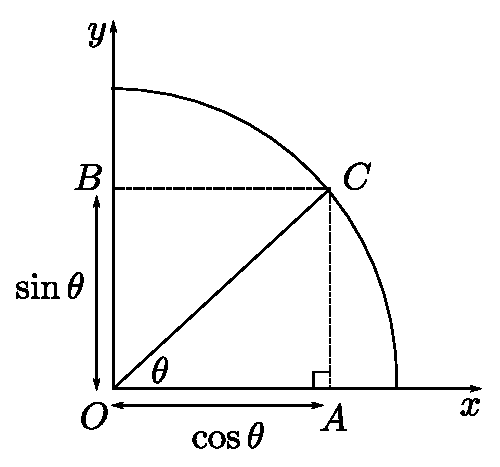
\includegraphics[scale=0.75]{img/cos-sin}
\caption{Geometric definition of $\cos$ and $\sin$, circle radius $r=OC=1$.}
\label{fig:cos-sin}
\end{figure}

\end{definition}

It can easily be seen that this definition is equivalent to the ``SOH CAH TOA" definition you are familiar with:

\begin{in_a_box}
$$\sin\theta=\frac{AC}{OC}=AC$$
$$\cos\theta=\frac{OA}{OC}=OA$$
$$\tan\theta=\frac{AC}{OA}=\frac{\sin\theta}{\cos\theta}$$
\end{in_a_box}

Although this definition allows for $\sin$, $\cos$ and $\tan$ to easily be extended to angles outside the range $\left[0,\frac{\pi}{2}\right]$

\subsection{Properties of sin, cos and tan}
\begin{thing}{Property}
$\cos^2\theta+\sin^2\theta=1$
\begin{proof}
Use Pythagoras' Theorem in triangle OAC.
\end{proof}
\end{thing}

\begin{thing}{Property}
$\cos$ and $\sin$ are periodic functions with period $2\pi$ (i.e. for any $x$, $\cos(x+2\pi)=\cos x$, $\sin(x+2\pi)=\sin x$).
\end{thing}

\begin{thing}{Property}
$\cos : \mathbb{R}\to[-1,1]$ and $\sin : \mathbb{R}\to[-1,1]$.
\end{thing}

\begin{figure}[H]
\centering
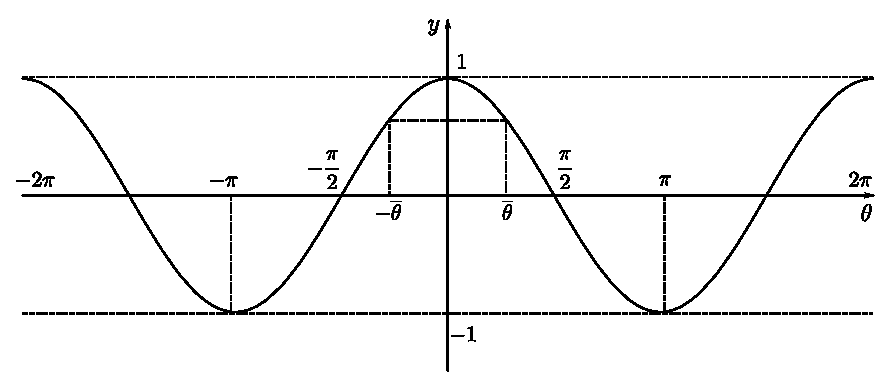
\includegraphics[scale=0.75]{img/cos}
\caption{Graph of $\cos\theta$.}
\label{fig:cos}
\end{figure}

\begin{figure}[H]
\centering
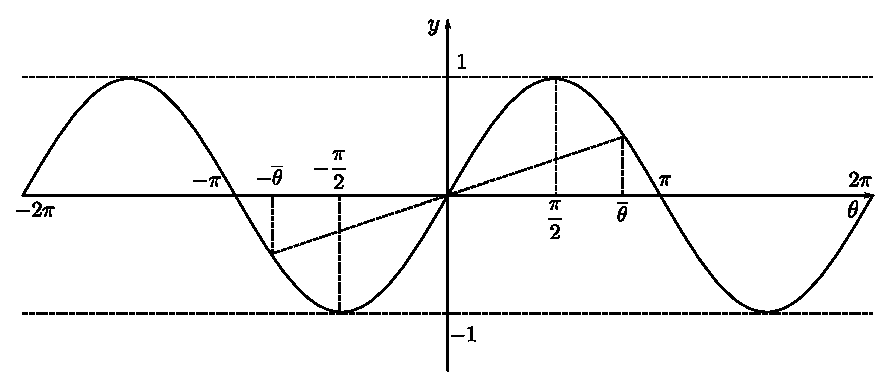
\includegraphics[scale=0.75]{img/sin}
\caption{Graph of $\sin\theta$.}
\label{fig:sin}
\end{figure}

\begin{thing}{Property}
$\cos$ is an even function. $\sin$ is an odd function.
\end{thing}

\begin{thing}{Property}
$\cos$ and $\sin$ are the same shape but shifted by $\pi/2$, which means
$$\cos\left(\theta-\frac{\pi}{2}\right)=\sin\theta$$
$$\sin\left(\theta+\frac{\pi}{2}\right)=\cos\theta$$
\end{thing}

\begin{thing}{Property: Addition formulae}
$$\cos(\theta+\phi)=\cos\theta\cos\phi-\sin\theta\sin\phi$$
$$\sin(\theta+\phi)=\sin\theta\cos\phi+\cos\theta\sin\phi$$
\end{thing}

\begin{thing}{Property: Double angle formulae}
$$\sin2\theta = 2\sin\theta\cos\theta$$
$$\cos2\theta = 1-2\sin^2\theta$$
$$\cos2\theta = 2\cos^2\theta-1$$
\begin{proof}
\begin{eqnarray*}
\cos 2\theta&=&\cos(\theta+\theta) \nonumber \\
&=& \cos^2\theta-\sin^2\theta \nonumber \\
&=& \cos^2\theta -(1-\cos^2\theta) \nonumber \\
&=& 2\cos^2\theta - 1 \nonumber \\
&=& 1-2\sin^2\theta
\end{eqnarray*}
\begin{eqnarray*}
\sin2\theta &=& \sin(\theta+\theta) \nonumber \\
&=& 2\sin\theta\cos\theta
\end{eqnarray*}
\end{proof}
\end{thing}

\begin{thing}{Property: Half angle formulae}
$$\cos^2\left(\frac{\alpha}{2}\right)=\frac{1+\cos\alpha}{2}$$
$$\sin^2\left(\frac{\alpha}{2}\right)=\frac{1-\cos\alpha}{2}$$
\begin{proof}
Let $2\theta=\alpha$, then
\begin{equation*}
\cos\alpha = 2\cos^2\left(\frac{\alpha}{2}\right) - 1 \quad \implies \quad \cos^2\left(\frac{\alpha}{2}\right)=\frac{1+\cos\alpha}{2}
\end{equation*}
\begin{equation*}
\cos\alpha = 1- 2\sin^2\left(\frac{\alpha}{2}\right) \quad \implies \quad \sin^2\left(\frac{\alpha}{2}\right)=\frac{1-\cos\alpha}{2}
\end{equation*}
\end{proof}
\end{thing}

\begin{thing}{Property}
$\tan$ has vertical asymptotes at $\theta=\frac{\pi}{2}\left(2N-1\right)$ for $N\in\mathbb{Z}$.
\begin{proof}
At $\theta=\frac{\pi}{2}\left(2N-1\right)$, $\cos\theta=0$.
\end{proof}
\end{thing}

\begin{thing}{Property}
$\tan : \mathbb{R}\setminus\{\frac{\pi}{2}(2N-1):N\in\mathbb{Z}\}\to\mathbb{R}$
\end{thing}

\begin{figure}[H]
\centering
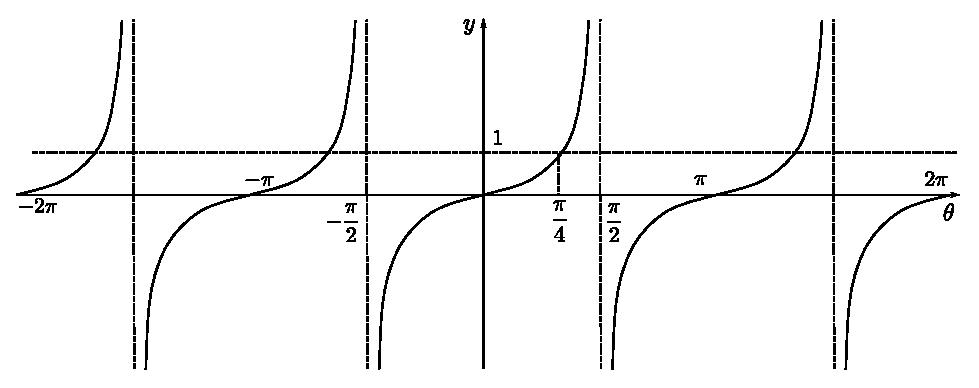
\includegraphics[scale=0.75]{img/tan}
\caption{Graph of $\tan\theta$.}
\label{fig:tan}
\end{figure}

\begin{thing}{Property}
$\tan$ is periodic with period $\pi$.
\end{thing}

\begin{thing}{Property: Double angle formula for $\tan$}
$$\tan(\theta+\phi)=\,\, \frac{\tan\theta+\tan\phi}{1-\tan\theta \tan\phi}$$
\begin{proof}
\begin{eqnarray*}
\tan(\theta+\phi)&=&\frac{\sin(\theta+\phi)}{\cos(\theta+\phi)} \nonumber \\
&=& \frac{\sin\theta\cos\phi+\cos\theta\sin\phi}{\cos\theta\cos\phi-\sin\theta\sin\phi}.
\end{eqnarray*}
Now divide by $\cos\theta\cos\phi$.
\end{proof}
\end{thing}

\begin{definition}{Secant, cosecant and cotangent}
The secant, cosecant and cotangent functions are defined as 
\[\sec x=\frac{1}{\cos x},\quad \mathrm{cosec} x=\frac{1}{\sin x},\quad \mathrm{cot} x=\frac{1}{\tan x}. \]
\end{definition}

\begin{thing}{Property}
$$1+\tan^2 x = \sec^2 x.$$
\begin{proof}
Divide \(\cos^2\theta+\sin^2\theta=1\) through by $\cos^2x$.
\end{proof}
\end{thing}

\begin{thing}{Property}
There are a number of ``special angles" for which you should remember the values of $\sin$, $\cos$ and $\tan$:

\begin{center}
\begin{tabular}{|c|c||c|c|c|}
\hline
\textbf{Angle (\degs)} & \textbf{Angle (\rads)} & \textbf{sin} & \textbf{cos} & \textbf{tan}\\\hline
0&0&0&1&0\\\hline
30&$\frac{\pi}{6}$&$\frac{1}{2}$&$\frac{\sqrt{3}}{2}$&$\frac{3}{\sqrt{3}}$\\\hline
45&$\frac{\pi}{4}$&$\frac{1}{\sqrt{2}}$&$\frac{1}{\sqrt{2}}$&1\\\hline
60&$\frac{\pi}{3}$&$\frac{\sqrt{3}}{2}$&$\frac{1}{2}$&$\sqrt{3}$\\\hline
90&$\frac{\pi}{2}$&1&0&$\infty$\\\hline
\end{tabular}
\end{center}
\end{thing}

These can be easily remembered via the following triangles:

\begin{figure}[H]
    \hspace{0.2cm}
    \subfigure[$\pi/4$ triangle.]{\label{fig:sin-cos-tan-45}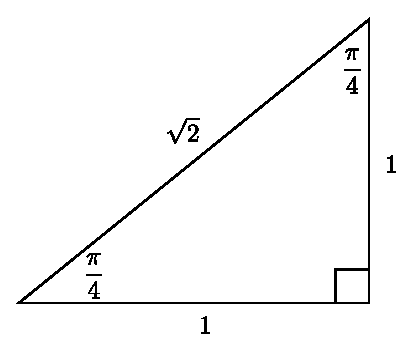
\includegraphics[scale=0.5]{img/sin-cos-tan-45}}
    \hspace{2.0cm}
    \subfigure[$\pi/3$, $\pi/6$ triangle.]{\label{fig:sin-cos-tan-30-60}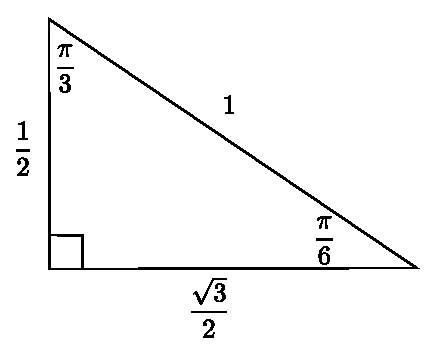
\includegraphics[scale=0.5]{img/sin-cos-tan-30-60}} \\
    \centering
  \caption{ Some well known results for particular angles can be derived by the above triangles for $\sin$, $\cos$ and $\tan$.}
  \label{fig:exponent-graphs}
\end{figure}

\section{Polar co-ordinates}
A circle with radius $r$ can be written as $x^2+y^2=r^2$. However, it is more natural to think of a circle as $r=\text{constant}$.

We can write a circle in this more natural way by using polar co-ordinates.

\begin{definition}
In \textbf{polar co-ordinates}, we give the distance from the origin, $r$, and the angle made with the $x$-axis, $theta$, as shown on the
diagram below.

\begin{figure}[H]
    \includegraphics[scale=0.5]{img/polar_def.jpg}
    \centering
  \caption{Polar co-ordinates are given by $r$ and $\theta$.}
\end{figure}

Shapes can be defined by writing $r$ in terms of $\theta$.
\end{definition}

The Cartesian (normal) co-ordinates can be written in terms of the polar co-ordinates:

\begin{in_a_box}
$$x=r\cos\theta$$
$$y=r\sin\theta$$
\end{in_a_box}

\begin{example}
The following cardiod can be most easily written in polar co-ordinates as $r=1-\cos\theta$.
\begin{figure}[H]
    \includegraphics[scale=0.5]{img/1-costheta.png}
    \centering
  \caption{The cardiod $r=1-\cos\theta$.}
\end{figure}

If written in Cartesian co-ordinates, it would be \[x^2+y^2+x=\sqrt{x^2+y^2}.\]

\end{example}
